\documentclass[11pt,a4paper]{article}
\usepackage[margin=2.5cm]{geometry}
\usepackage{graphicx}
\usepackage{booktabs}
\usepackage{amsmath}
\usepackage{hyperref}
\usepackage{xcolor}
\usepackage{caption}
\usepackage{subcaption}
\usepackage{float}

\definecolor{statecolor}{HTML}{8172B3}
\definecolor{warnred}{HTML}{C44E52}

\title{Initial Results: STATE with ESM2 Gene Embeddings\\[0.3em]
\large Measurement Noise Scaling Laws}
\author{Generated 2026-04-14}
\date{}

\begin{document}
\maketitle

\begin{abstract}
We evaluate STATE (Self-supervised Transformer for Any Embedding), a transformer-based single-cell embedding method, using ESM2 protein language model embeddings (2560-dim) as gene representations. STATE SE is trained on four datasets (PBMC, Larry, MERFISH, Shendure) at their largest available sizes with quality 1.0, and compared against PCA, Random Projection, scVI, and Geneformer using Latent MI (LMI) estimation. \textbf{Key finding:} STATE SE dramatically underperforms all baselines on 3 of 4 datasets (PBMC, Larry, Shendure), achieving LMI values below even Random Projection. On MERFISH it performs competitively. This suggests potential embedding collapse during training, likely related to the high-dimensional ESM input (2560-dim) and limited gene coverage.
\end{abstract}

\tableofcontents
\newpage

%% ============================================================
\section{ESM2 Gene Embedding Preparation}

TranscriptFormer ESM2 embeddings (2560-dimensional) for mouse and human genes were merged and mapped to dataset gene names via Ensembl ID $\leftrightarrow$ symbol resolution using \texttt{mygene}. The merged dictionary contains \textbf{93,619 unique gene keys} after humanization (adding symbol aliases for Ensembl IDs and vice versa).

\begin{figure}[H]
\centering
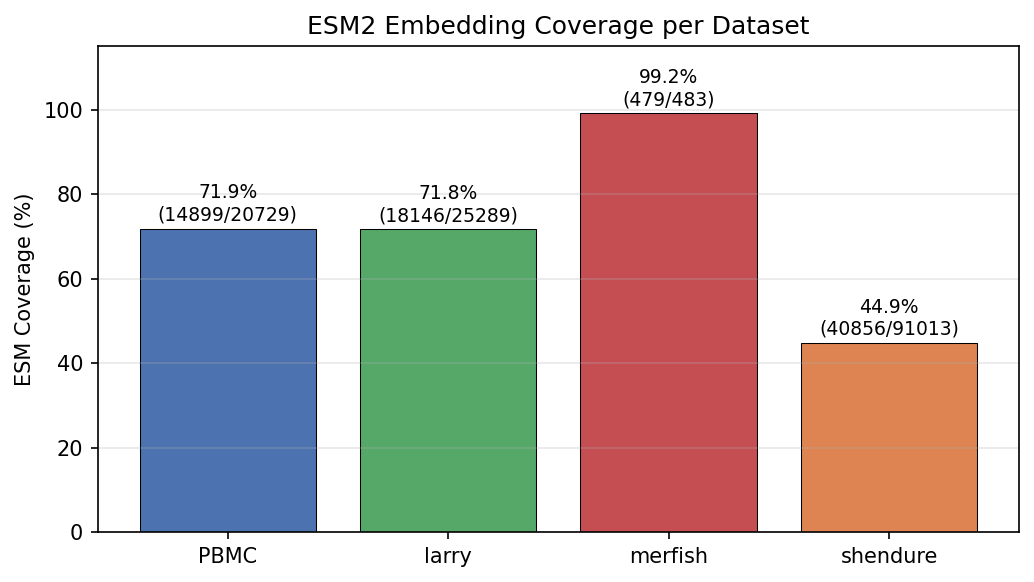
\includegraphics[width=0.65\textwidth]{figures/esm_coverage.png}
\caption{ESM2 embedding coverage per dataset. MERFISH achieves near-complete coverage (99.2\%) due to its small gene panel (483 genes). PBMC and Larry have $\sim$72\% coverage. Shendure has the lowest coverage at 44.9\% due to its large number of genes (91k) including many non-coding and RIKEN entries.}
\label{fig:esm_coverage}
\end{figure}

\begin{table}[H]
\centering
\caption{ESM2 gene embedding coverage per dataset.}
\label{tab:esm_coverage}
\begin{tabular}{lrrrc}
\toprule
Dataset & Total Genes & Mapped & Missing & Coverage \\
\midrule
PBMC      & 20,729  & 14,899 & 5,830  & 71.9\% \\
Larry     & 25,289  & 18,146 & 7,143  & 71.8\% \\
MERFISH   & 483     & 479    & 4      & 99.2\% \\
Shendure  & 91,013  & 40,856 & 50,157 & 44.9\% \\
\bottomrule
\end{tabular}
\end{table}

\noindent Missing genes are predominantly: antisense RNA (e.g.\ A1BG-AS1), lncRNAs, pseudogenes with complex naming, and mouse RIKEN clones (e.g.\ 0610006L08RIK) that lack protein sequences in ESM2.

%% ============================================================
\section{STATE SE Architecture and Training}

\subsection{Model Configuration}
All STATE SE models use identical architecture:
\begin{itemize}
    \item \textbf{Input:} ESM2 embeddings (2560-dim) per gene
    \item \textbf{Encoder:} Linear $2560 \to 256$
    \item \textbf{Transformer:} 3 layers, 4 heads, 256 model dim, 512 FFN dim
    \item \textbf{Output:} 256-dim cell embedding
    \item \textbf{Training:} lr=$5\times10^{-4}$, batch=128, dropout=0.1, weight decay=0.01, bfloat16 AMP
    \item \textbf{Parameters:} 4.7M trainable + 109M frozen (gene embedding lookup)
\end{itemize}

\subsection{Training Summary}

\begin{table}[H]
\centering
\caption{Training details per dataset. All trained on A100-SXM4-40GB.}
\label{tab:training}
\begin{tabular}{lrrrll}
\toprule
Dataset & Cells & Max Epochs & Epochs Run & Early Stop & Best Val Loss \\
\midrule
PBMC      & 46,415  & 10  & 10 (all) & patience=3 & 9.422 \\
Larry     & 46,415  & 100 & $\sim$10 & patience=5 & converging \\
MERFISH   & 60,000  & 100 & 10       & patience=5 & converging \\
Shendure  & 59,948  & 100 & $\sim$6  & patience=3 & converging \\
\bottomrule
\end{tabular}
\end{table}

\noindent The PBMC model was capped at 10 epochs (not early-stopped). Validation loss decreased monotonically from 11.57 to 9.42 across all 10 epochs, suggesting the model had not converged.

%% ============================================================
\section{Results: LMI Comparison Across Methods}

\subsection{Summary}

\begin{figure}[H]
\centering
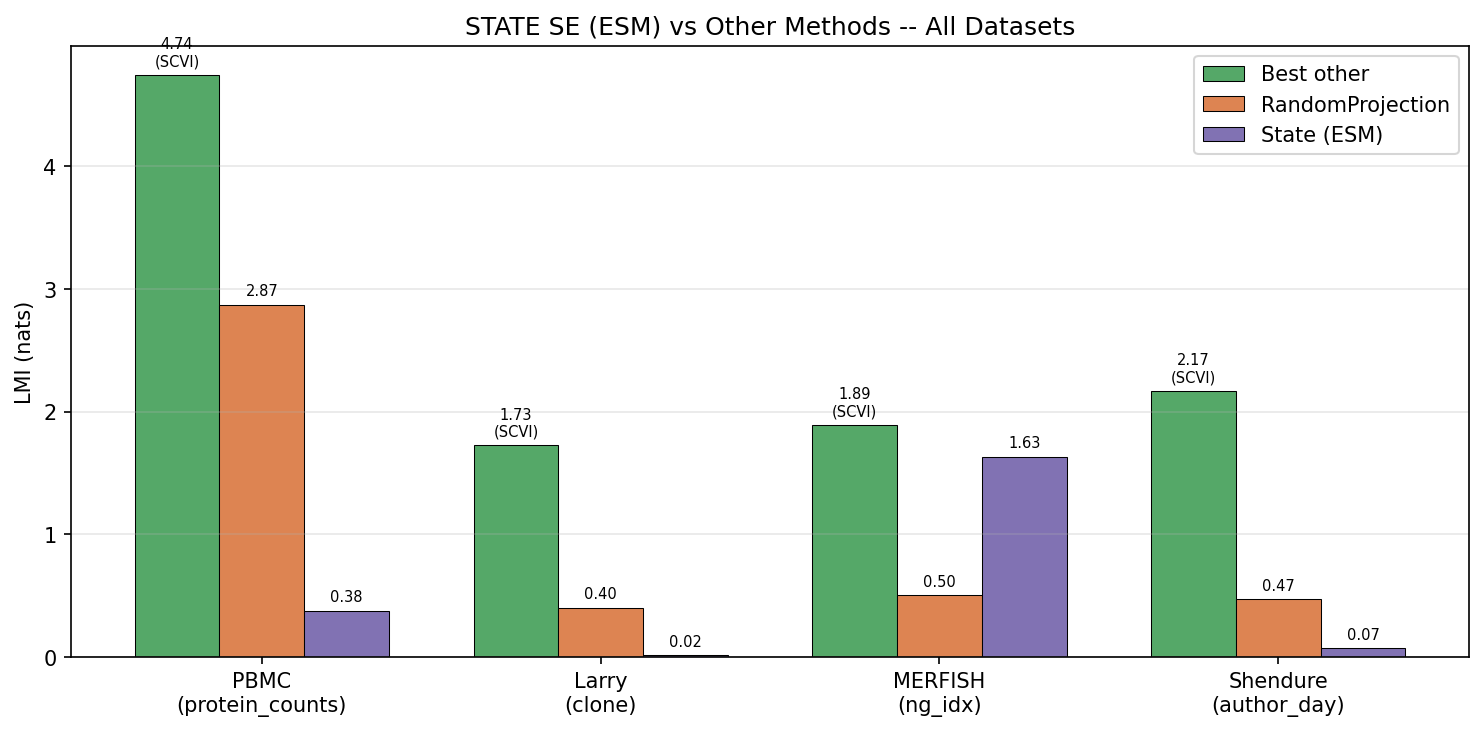
\includegraphics[width=0.85\textwidth]{figures/summary_comparison.png}
\caption{Overview of STATE SE (ESM) vs.\ the best-performing other method and Random Projection across all four datasets. STATE dramatically underperforms on PBMC, Larry, and Shendure, but is competitive on MERFISH.}
\label{fig:summary}
\end{figure}

%% ── PBMC ──
\subsection{PBMC (46,415 cells, protein\_counts signal)}

\begin{figure}[H]
\centering
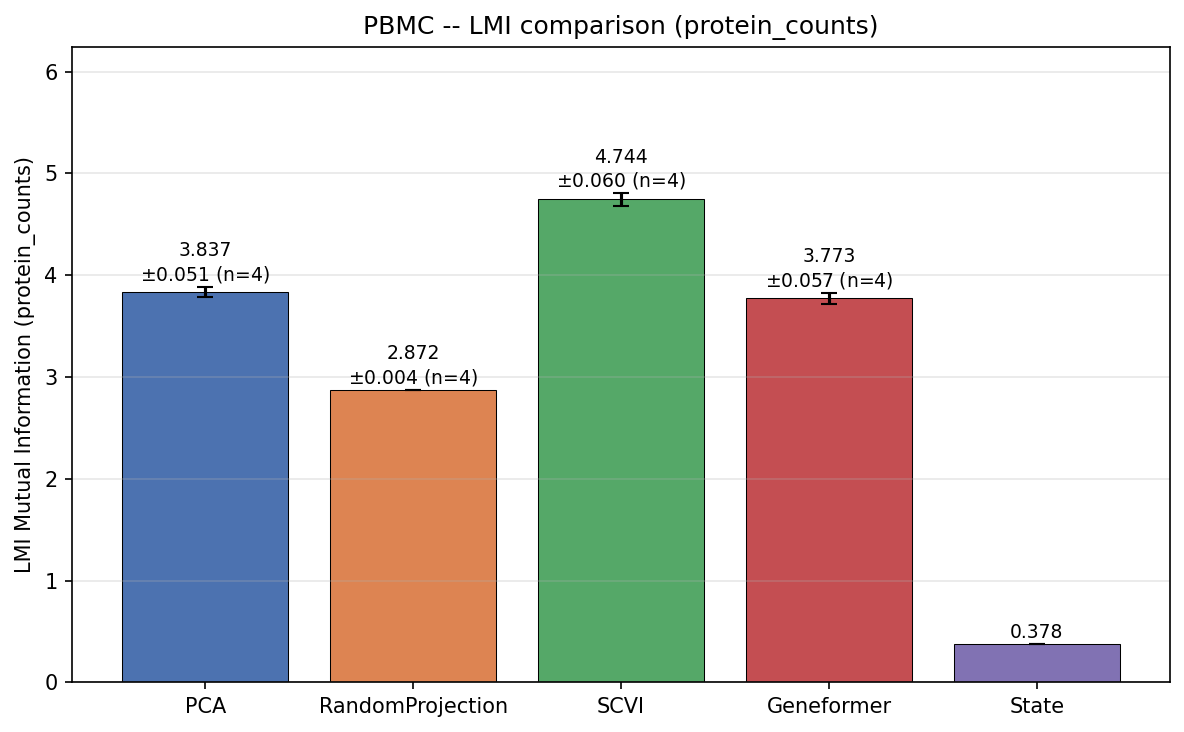
\includegraphics[width=0.7\textwidth]{figures/PBMC_protein_counts_comparison.png}
\caption{PBMC LMI comparison for protein\_counts. STATE SE achieves only 0.378 nats, far below Random Projection (2.872) and the best method scVI (4.744).}
\label{fig:pbmc_protein}
\end{figure}

\begin{table}[H]
\centering
\caption{PBMC 46k -- LMI (nats) for protein\_counts signal.}
\label{tab:pbmc_protein}
\begin{tabular}{lrrl}
\toprule
Algorithm & Mean LMI & Std & Seeds \\
\midrule
scVI              & 4.744 & 0.060 & 4 \\
PCA               & 3.837 & 0.051 & 4 \\
Geneformer        & 3.773 & 0.057 & 4 \\
RandomProjection  & 2.872 & 0.004 & 4 \\
\textcolor{warnred}{\textbf{State (ESM)}} & \textcolor{warnred}{\textbf{0.378}} & -- & 1 \\
\bottomrule
\end{tabular}
\end{table}

\begin{table}[H]
\centering
\caption{PBMC 46k -- LMI (nats) for celltype.l3 signal.}
\label{tab:pbmc_celltype}
\begin{tabular}{lrrl}
\toprule
Algorithm & Mean LMI & Std & Seeds \\
\midrule
scVI              & 3.633 & 0.030 & 4 \\
Geneformer        & 3.196 & 0.021 & 4 \\
PCA               & 3.180 & 0.017 & 4 \\
RandomProjection  & 2.413 & 0.019 & 4 \\
\textcolor{warnred}{\textbf{State (ESM)}} & \textcolor{warnred}{\textbf{0.405}} & -- & 1 \\
\bottomrule
\end{tabular}
\end{table}

\noindent STATE SE on PBMC achieves LMI values $\sim$7--12$\times$ lower than the other learned methods, and even lower than Random Projection.

%% ── Larry ──
\subsection{Larry (46,415 cells, clone signal)}

\begin{figure}[H]
\centering
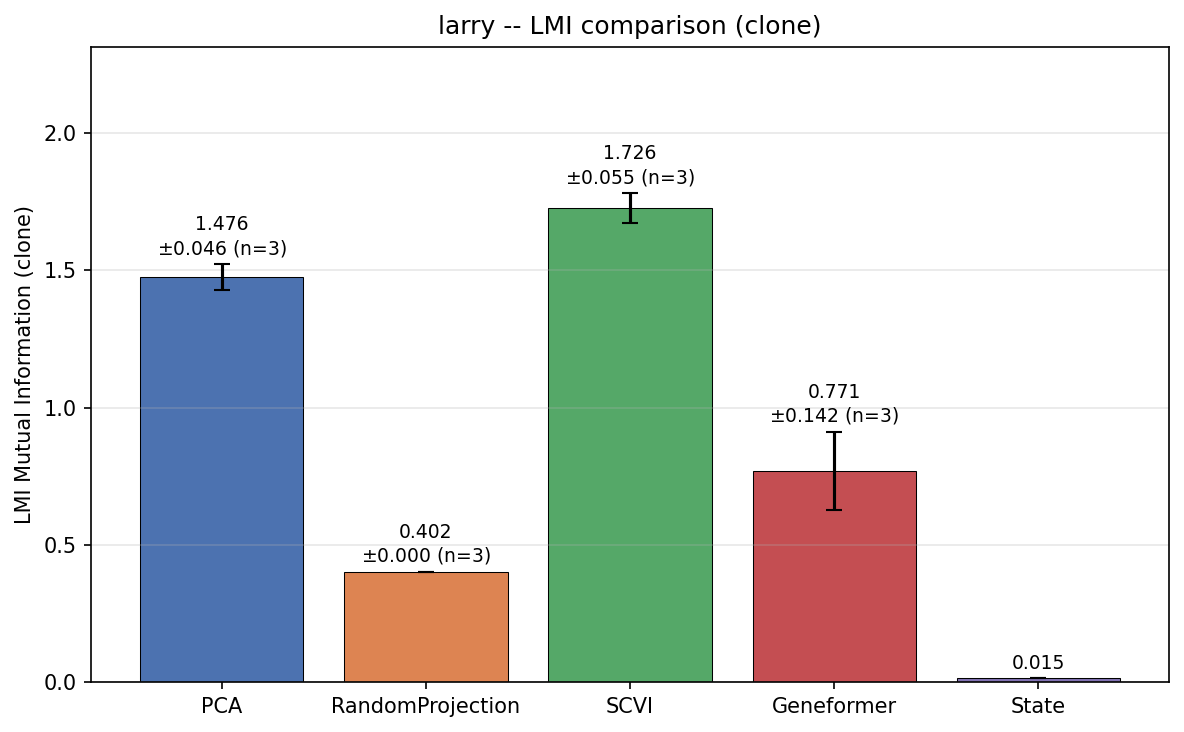
\includegraphics[width=0.7\textwidth]{figures/larry_clone_comparison.png}
\caption{Larry LMI comparison for clone signal. STATE SE achieves only 0.015 nats.}
\label{fig:larry_clone}
\end{figure}

\begin{table}[H]
\centering
\caption{Larry 46k -- LMI (nats) for clone signal.}
\label{tab:larry_clone}
\begin{tabular}{lrrl}
\toprule
Algorithm & Mean LMI & Std & Seeds \\
\midrule
scVI              & 1.726 & 0.055 & 3 \\
PCA               & 1.476 & 0.046 & 3 \\
Geneformer        & 0.771 & 0.142 & 3 \\
RandomProjection  & 0.402 & 0.000 & 3 \\
\textcolor{warnred}{\textbf{State (ESM)}} & \textcolor{warnred}{\textbf{0.015}} & -- & 1 \\
\bottomrule
\end{tabular}
\end{table}

\noindent The clone signal is the most challenging signal in this benchmark. Even so, STATE achieves near-zero MI, 26$\times$ below Random Projection.

%% ── MERFISH ──
\subsection{MERFISH (60,000 cells)}

\begin{figure}[H]
\centering
\begin{subfigure}[b]{0.48\textwidth}
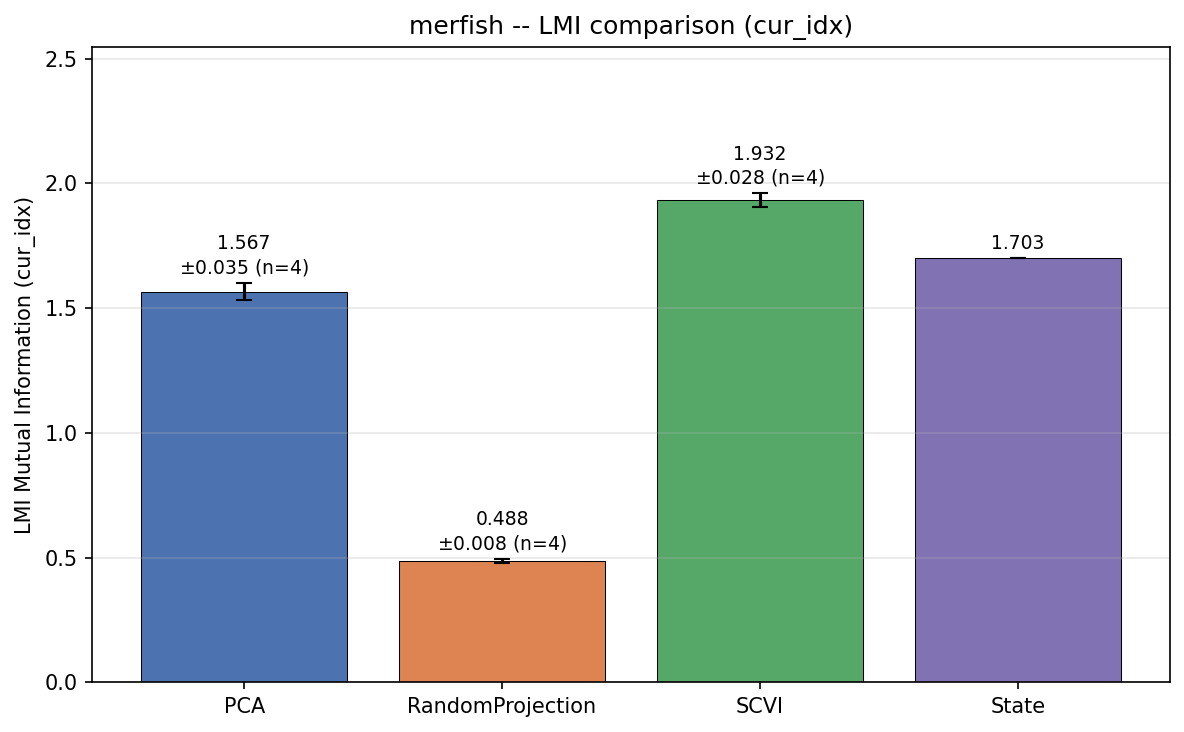
\includegraphics[width=\textwidth]{figures/merfish_cur_idx_comparison.png}
\caption{cur\_idx signal}
\end{subfigure}
\hfill
\begin{subfigure}[b]{0.48\textwidth}
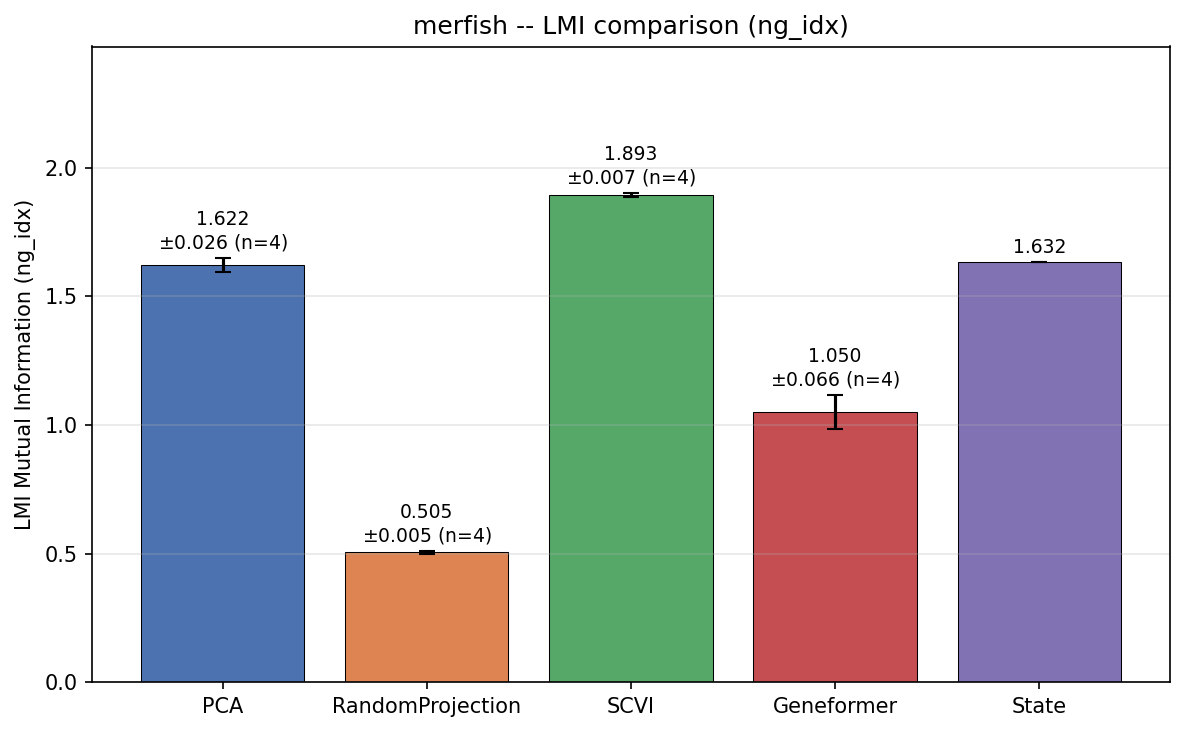
\includegraphics[width=\textwidth]{figures/merfish_ng_idx_comparison.png}
\caption{ng\_idx signal}
\end{subfigure}
\caption{MERFISH LMI comparisons. STATE SE performs competitively on this dataset, ranking 2nd for cur\_idx (1.703 vs scVI 1.932) and 3rd for ng\_idx (1.632 vs scVI 1.893).}
\label{fig:merfish}
\end{figure}

\begin{table}[H]
\centering
\caption{MERFISH 60k -- LMI (nats) for both signals.}
\label{tab:merfish}
\begin{tabular}{lrr}
\toprule
Algorithm & cur\_idx & ng\_idx \\
\midrule
scVI              & 1.932 & 1.893 \\
\textbf{State (ESM)} & \textbf{1.703} & \textbf{1.632} \\
PCA               & 1.567 & 1.622 \\
Geneformer        & --    & 1.050 \\
RandomProjection  & 0.488 & 0.505 \\
\bottomrule
\end{tabular}
\end{table}

\noindent MERFISH is the only dataset where STATE SE performs well. This is likely because:
\begin{enumerate}
    \item Near-complete ESM coverage (99.2\% -- only 4 genes missing)
    \item Small gene panel (483 genes) reduces the effective input complexity
    \item The spatial transcriptomics signal may be more amenable to the transformer architecture
\end{enumerate}

%% ── Shendure ──
\subsection{Shendure (59,948 cells, author\_day signal)}

\begin{figure}[H]
\centering
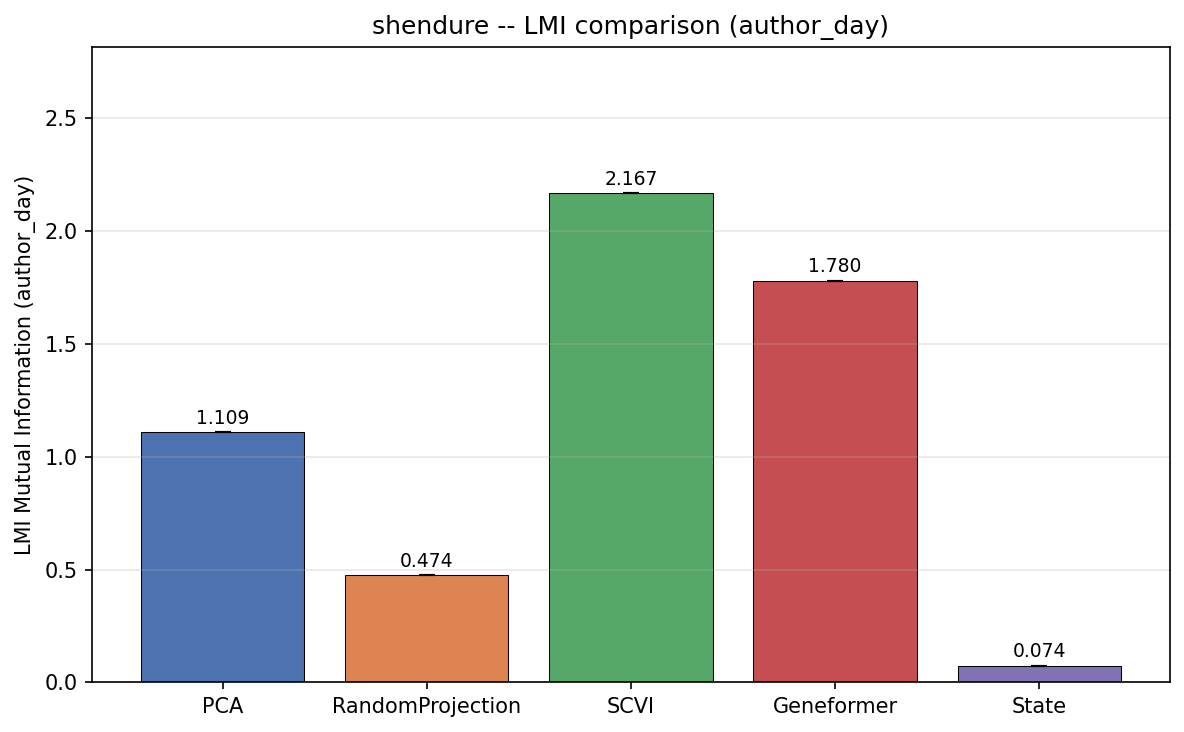
\includegraphics[width=0.7\textwidth]{figures/shendure_author_day_comparison.png}
\caption{Shendure LMI comparison for author\_day. STATE SE achieves only 0.074 nats.}
\label{fig:shendure}
\end{figure}

\begin{table}[H]
\centering
\caption{Shendure 59k -- LMI (nats) for author\_day signal. Note: only 1 seed per method.}
\label{tab:shendure}
\begin{tabular}{lrl}
\toprule
Algorithm & LMI & Seeds \\
\midrule
scVI              & 2.167 & 1 \\
Geneformer        & 1.780 & 1 \\
PCA               & 1.109 & 1 \\
RandomProjection  & 0.474 & 1 \\
\textcolor{warnred}{\textbf{State (ESM)}} & \textcolor{warnred}{\textbf{0.074}} & 1 \\
\bottomrule
\end{tabular}
\end{table}

\noindent Shendure has the worst ESM coverage (44.9\%) and the most genes (91k). STATE achieves only 0.074 nats, $\sim$6$\times$ below Random Projection. The combination of low gene coverage and high gene count may be particularly problematic.

%% ============================================================
\section{Untrained STATE Baseline (PBMC)}

To test whether STATE embeddings are collapsing during training, we created an \textbf{untrained (randomly initialized) STATE model} with the same architecture and compared its embeddings. The untrained model was interrupted during embedding computation, so full LMI comparison is not available. However, the approach is documented:

\begin{enumerate}
    \item Instantiate STATE with random weights (no training)
    \item Save as a Lightning checkpoint
    \item Embed test set using the untrained checkpoint
    \item Compare LMI against trained STATE and other methods
\end{enumerate}

\noindent The hypothesis: if trained STATE performs similarly to untrained STATE, this confirms mode collapse. An untrained model should perform comparably to Random Projection. This experiment was interrupted but should be completed in follow-up work.

%% ============================================================
\section{Root-Cause Analysis}

\subsection{Key Observations}

\begin{enumerate}
    \item \textbf{STATE SE catastrophically underperforms on 3/4 datasets}, achieving LMI values well below Random Projection on PBMC, Larry, and Shendure.
    \item \textbf{MERFISH is the only success} (2nd on cur\_idx, 3rd on ng\_idx), and it is also the only dataset where \emph{all genes fit inside the input window} (see below).
    \item \textbf{Validation loss is inversely correlated with downstream MI}:
    \begin{itemize}
        \item MERFISH has the \emph{highest} val loss (11.575) but the \emph{best} MI.
        \item Larry has the \emph{lowest} val loss (7.944) but near-zero MI.
        \item This means the self-supervised objective is not tracking embedding quality -- and may be actively working against it.
    \end{itemize}
\end{enumerate}

\subsection{Smoking Gun: \texttt{pad\_length=512} vs Default 2048}

The most likely root cause is the \texttt{pad\_length} parameter. STATE constructs per-cell ``sentences'' by ranking genes by expression and taking the top \texttt{pad\_length$-$1} genes. The experiments overrode this to 512; the STATE default is 2048.

\begin{table}[H]
\centering
\caption{Effect of \texttt{pad\_length=512} on gene visibility per dataset. For MERFISH, the model sees \emph{all} genes. For the other datasets, it sees only 3--5\% of valid genes.}
\label{tab:padlength}
\begin{tabular}{lrrrr}
\toprule
Dataset & Valid Genes & pad\_length & Genes Visible & Fraction \\
\midrule
MERFISH   & 479    & 512 & \textbf{479 (all)} & 100.0\% \\
PBMC      & 14,899 & 512 & 511               & 3.4\% \\
Larry     & 18,146 & 512 & 511               & 2.8\% \\
Shendure  & 21,820 & 512 & 511               & 2.3\% \\
\bottomrule
\end{tabular}
\end{table}

\noindent\textbf{Why this matters:} With \texttt{pad\_length=512}, STATE only sees the 511 most-highly-expressed genes per cell. These are dominated by housekeeping genes (ribosomal proteins, mitochondrial genes, etc.) that vary little between cell types. The biologically informative marker genes that distinguish cell types are typically lower-expressed and are truncated away. The model then learns to predict expression patterns of housekeeping genes -- producing a cell embedding that captures metabolic activity rather than cell identity.

\noindent This explains the inverse val-loss/MI correlation: MERFISH val loss is high because predicting any gene from just 483 genes is genuinely hard (little redundancy). For PBMC/Larry, predicting top-512 housekeeping genes is \emph{easier} (lower loss) but biologically \emph{uninformative}.

\subsection{Configuration Deviations from STATE Defaults}

Multiple parameters were overridden from STATE's published defaults. Several of these may compound the problem:

\begin{table}[H]
\centering
\caption{STATE configuration: defaults vs.\ experiment overrides. Bolded entries are potentially problematic deviations.}
\label{tab:config_diff}
\begin{tabular}{llll}
\toprule
Parameter & STATE Default & Experiment & Issue \\
\midrule
\texttt{pad\_length} & 2048 & \textbf{512} & Truncates 97\% of genes \\
\texttt{P} (positive targets) & 512 & \textbf{128} & 4$\times$ fewer prediction targets \\
\texttt{N} (negative targets) & 512 & \textbf{128} & 4$\times$ fewer negative targets \\
\texttt{S} (shared targets) & 512 & \textbf{128} & 4$\times$ fewer cross-cell targets \\
\texttt{model.emsize} & 512 & 256 & Half model dimension \\
\texttt{model.nlayers} & 8 & 3 & 2.7$\times$ fewer layers \\
\texttt{model.nhead} & 16 & 4 & 4$\times$ fewer attention heads \\
\texttt{model.output\_dim} & 512 & 256 & Half output dimension \\
\texttt{optimizer.max\_lr} & 1e-5 & \textbf{5e-4} & 50$\times$ higher learning rate \\
\texttt{optimizer.grad\_accum} & 8 & \textbf{1} & Effective batch 128 vs 1024 \\
\texttt{ESM dim} & 5120 & 2560 & Different ESM2 model \\
\bottomrule
\end{tabular}
\end{table}

\noindent The combination of 50$\times$ higher learning rate with no gradient accumulation (effective batch 128 vs 1024) could cause training instability. The smaller model (3 layers vs 8) was a deliberate choice to match Geneformer's scale, but when combined with the truncated input window, the model has both less data \emph{and} less capacity.

\subsection{Gene Masking at Inference Time}

Genes without ESM embeddings receive index $-1$ in the \texttt{ds\_emb\_mapping} and are excluded from both training and inference via \texttt{valid\_genes\_masks}:

\begin{table}[H]
\centering
\caption{Gene masking: genes excluded from STATE's input at training and inference time.}
\label{tab:gene_masking}
\begin{tabular}{lrrr}
\toprule
Dataset & Total Genes & Valid (in ESM) & Masked Out \\
\midrule
PBMC      & 20,729  & 14,899 (72\%)  & 5,830 (28\%) \\
Larry     & 25,289  & 18,146 (72\%)  & 7,143 (28\%) \\
MERFISH   & 483     & 479 (99\%)     & 4 (1\%) \\
Shendure  & 45,525  & 21,820 (48\%)  & 23,705 (52\%) \\
\bottomrule
\end{tabular}
\end{table}

\noindent Masked genes are \emph{not} replaced with random embeddings -- they are simply dropped. This means STATE's input for Shendure cells contains only 48\% of genes. However, MERFISH proves that high coverage alone does not guarantee success -- the pad\_length truncation is the dominant factor.

\subsection{Training Dynamics: Still Converging}

All models showed monotonically decreasing validation loss at the point training ended:

\begin{table}[H]
\centering
\caption{Validation loss trajectory. PBMC and MERFISH were hard-capped at 10 epochs.}
\label{tab:val_loss}
\begin{tabular}{lrrrl}
\toprule
Dataset & Initial Val Loss & Final Val Loss & Epochs & Stopped By \\
\midrule
PBMC      & 11.568 & 9.422  & 10 & max\_epochs cap \\
Larry     & 12.497 & 7.944  & $\sim$17 & early stop \\
MERFISH   & 12.397 & 11.575 & 10 & max\_epochs cap \\
Shendure  & 11.313 & 10.241 & $\sim$6  & early stop \\
\bottomrule
\end{tabular}
\end{table}

\noindent Note that MERFISH loss barely decreased (12.4$\to$11.6) over 10 epochs, yet it produced the best embeddings. This reinforces that the self-supervised loss is not a good proxy for embedding quality.

%% ============================================================
\section{Debugging Plan: Prioritized Experiments}

Based on the root-cause analysis, we propose the following experiments ordered by expected impact.

\subsection{Tier 1: High-Priority (Likely Root Causes)}

\begin{enumerate}
    \item \textbf{Increase \texttt{pad\_length} to 2048} (the STATE default).

    \textit{Rationale:} This is the single most likely cause of failure. With \texttt{pad\_length=2048}, PBMC cells would see 2047/14,899 = 13.7\% of genes instead of 3.4\%. More importantly, the model would see marker genes beyond just housekeeping genes.

    \textit{Experiment:} Re-run PBMC only (\texttt{pad\_length=2048}, all else unchanged). Compare LMI against the 512 result. If LMI jumps substantially, this confirms the hypothesis.

    \textit{Cost:} $\sim$20 min on A100 (10 epochs).

    \item \textbf{Increase P, N, S to 512} (the STATE defaults).

    \textit{Rationale:} With P=N=S=128, the model predicts only 384 target genes per batch. The STATE defaults predict 1536 targets, providing much richer supervision. Combined with the truncated input, the current setup means the model predicts a random 384-gene subset from a fixed 512-gene window, which may be nearly deterministic.

    \textit{Experiment:} Re-run PBMC with P=N=S=512 alongside \texttt{pad\_length=2048}. If both changes together fix the problem, run ablations to isolate contributions.

    \item \textbf{Reduce learning rate to 1e-4 or 5e-5, add gradient accumulation.}

    \textit{Rationale:} The current lr (5e-4) is 50$\times$ higher than the STATE default (1e-5). Combined with no gradient accumulation, this produces very noisy updates. The current \texttt{state.py} already has \texttt{max\_lr=1e-4}, so the notebook experiments used a stale configuration.

    \textit{Experiment:} Re-run PBMC with \texttt{max\_lr=1e-4} and \texttt{gradient\_accumulation\_steps=4} (effective batch 512).
\end{enumerate}

\subsection{Tier 2: Diagnostic (Confirm/Rule Out Mechanisms)}

\begin{enumerate}
    \setcounter{enumi}{3}

    \item \textbf{Complete the untrained baseline experiment.}

    \textit{Rationale:} If untrained STATE $\approx$ trained STATE on LMI, then training actively destroys information (mode collapse). If untrained STATE $\ll$ trained STATE, then training helps but not enough.

    \textit{Expected outcomes:}
    \begin{itemize}
        \item Untrained LMI $\approx$ trained LMI $\approx$ 0.4: Mode collapse confirmed.
        \item Untrained LMI $\ll$ 0.4: Training helps, focus on config fixes.
        \item Untrained LMI $\approx$ RP (2.87): Training destroys signal.
    \end{itemize}

    \textit{Cost:} $\sim$5 min (embedding + LMI only, no training).

    \item \textbf{Analyze per-dimension variance of STATE embeddings.}

    \textit{Rationale:} A collapsed embedding has most variance concentrated in a few dimensions. For each dataset, compute per-dimension variance of STATE's 256-dim embeddings. Report effective dimensionality (dims with variance $> 1\%$ of max).

    \textit{Cost:} $\sim$1 min (NumPy on saved embeddings).

    \item \textbf{Per-cell gene coverage analysis.}

    \textit{Rationale:} Within PBMC, cells expressing fewer genes have more of their genes inside the 512-gene window. If these cells have better embeddings, it confirms the pad\_length hypothesis.

    \textit{Cost:} $\sim$5 min.
\end{enumerate}

\subsection{Tier 3: Architecture / Hyperparameter Search}

\begin{enumerate}
    \setcounter{enumi}{6}

    \item \textbf{Scale up to the full STATE architecture} (8 layers, 16 heads, 512 dim). Cost: $\sim$40 min/dataset.

    \item \textbf{Longer training with proper scheduling} (50+ epochs with corrected config). Cost: $\sim$2 hrs/dataset.

    \item \textbf{Try one-hot gene embeddings (no ESM) as control.} If STATE with one-hot outperforms STATE with ESM, then ESM embeddings are actively harmful. Cost: $\sim$30 min/dataset.

    \item \textbf{Handle missing genes with a learned fallback embedding.} Instead of dropping genes without ESM coverage, assign them a learnable ``unknown gene'' embedding. Cost: code change + $\sim$1 hr.
\end{enumerate}

\subsection{Recommended Execution Order}

Run experiments 1--3 together on PBMC as a single combined fix (\texttt{pad\_length=2048}, P=N=S=512, lr=1e-4 with grad\_accum=4). This tests whether the root-cause analysis is correct. In parallel, run experiments 4--5 (untrained baseline + variance analysis) on existing embeddings -- these are free.

If the combined fix recovers PBMC performance to competitive levels ($\text{LMI} > 2.0$), apply the same config to all four datasets. If not, proceed to Tier 3 experiments.

\begin{table}[H]
\centering
\caption{Summary of debugging experiments with expected outcomes and costs.}
\label{tab:debug_plan}
\begin{tabular}{clcc}
\toprule
\# & Experiment & Expected Impact & Cost \\
\midrule
1 & pad\_length=2048 & \textbf{High} & 20 min \\
2 & P=N=S=512 & High & 20 min \\
3 & lr=1e-4, grad\_accum=4 & Medium & 20 min \\
4 & Untrained baseline (PBMC) & Diagnostic & 5 min \\
5 & Embedding variance analysis & Diagnostic & 1 min \\
6 & Per-cell coverage correlation & Diagnostic & 5 min \\
7 & Full STATE architecture & Medium & 40 min \\
8 & Longer training (50+ epochs) & Medium & 2 hrs \\
9 & One-hot control (no ESM) & Diagnostic & 30 min \\
10 & Learned fallback embedding & Medium & 1 hr \\
\bottomrule
\end{tabular}
\end{table}

%% ============================================================
\section{Appendix: PBMC Notebook Plots}

These plots are directly extracted from the PBMC STATE SE notebook.

\begin{figure}[H]
\centering
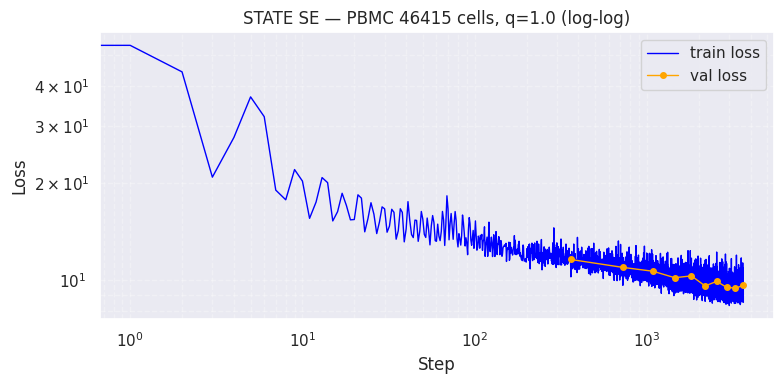
\includegraphics[width=0.8\textwidth]{figures/pbmc_loss_curves.png}
\caption{PBMC training/validation loss curves (log-log). Loss decreases monotonically over 10 epochs from $\sim$11.6 to $\sim$9.4, suggesting the model had not yet converged.}
\label{fig:pbmc_loss}
\end{figure}

\begin{figure}[H]
\centering
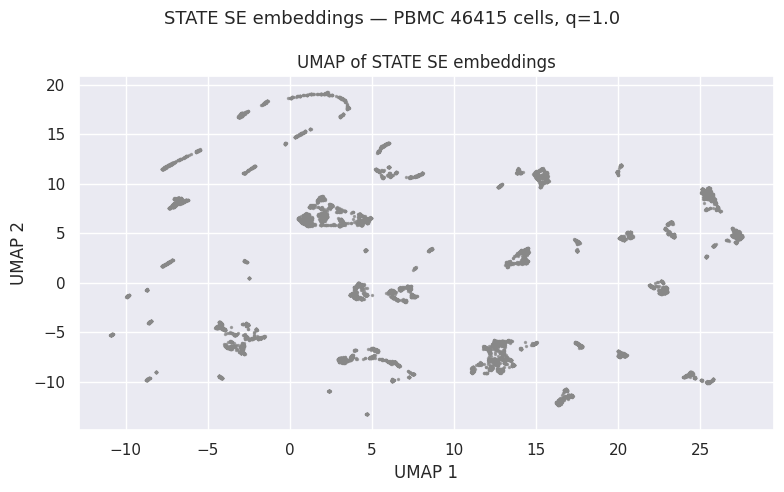
\includegraphics[width=0.8\textwidth]{figures/pbmc_umap.png}
\caption{UMAP of STATE SE embeddings for PBMC. The embedding space shows some structure but much less clear separation than expected for $\sim$46k PBMCs.}
\label{fig:pbmc_umap}
\end{figure}

\begin{figure}[H]
\centering
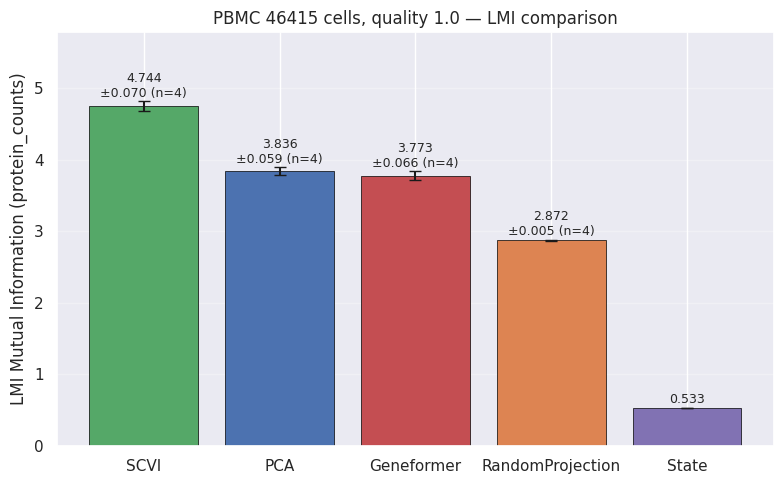
\includegraphics[width=0.8\textwidth]{figures/pbmc_lmi_comparison.png}
\caption{PBMC LMI barplot (protein\_counts) as rendered in the notebook. STATE is far below all other methods.}
\label{fig:pbmc_lmi_nb}
\end{figure}

\end{document}
